\graphicspath{{chapters/02/}}
\chapter{scRNA-seq backstage}


\hypertarget{challenges-in-single-cell-workflow}{%
\section{Challenges in single cell
workflow}\label{challenges-in-single-cell-workflow}}

\begin{figure}
\centering
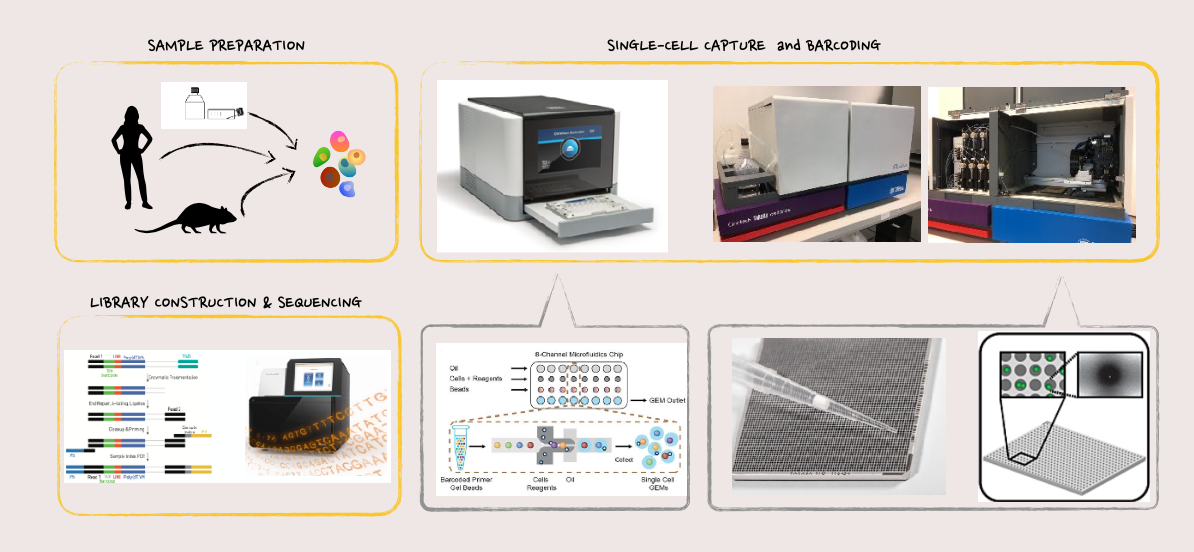
\includegraphics[width=0.5\textwidth]{images/Screenshot.png}
\caption{}
\end{figure}

\hypertarget{sources-of-experimental-variability}{%
\subsection{Sources of experimental
variability}\label{sources-of-experimental-variability}}

\begin{enumerate}
\def\labelenumi{\arabic{enumi}.}
\tightlist
\item
  human factor
\item
  cell suspension preparation
\item
  cDNA synthesis
\item
  PCR
\item
  NGS
\end{enumerate}

\hypertarget{single-cell-suspension}{%
\subsection{Single-cell suspension}\label{single-cell-suspension}}

RNA degrades very fast, so it is required to quickly transfer separated
samples to the sequencing machine. A good quality single-cell suspension
should have high viability, no dead or dying cells, cell debris removed
and unaltered transcriptional profile.

Fresh samples can be obtained from:

\begin{itemize}
\tightlist
\item
  suspension cell lines e.g.~blood
\item
  adherent cell lines → trypsin digestion is usually applied for
  dissociation, but it is possible to choose among other enzymes
  e.g.~Accutase or TrypLe. It is then necessary to resuspend cells to
  avoid aggregates. Wide-pore tips are used to avoid pression and stress
  induction, leading to an overall higher cell survival.
\item
  dissociation of tissues
\end{itemize}

Cells are different in size, gene expression profile and are
characterized by peculiar extracellular matrix composition, which
affects dissociation techniques.

\hypertarget{single-cell-suspension-from-solid-tissue}{%
\subsubsection{Single cell suspension from solid
tissue}\label{single-cell-suspension-from-solid-tissue}}

\begin{enumerate}
\def\labelenumi{\arabic{enumi}.}
\tightlist
\item
  tissue dissection
\item
  rinse with PBS to get rid of unwanted components
\item
  mechanical dissociation to increase the contact area with cell and
  enzyme
\item
  add digestive enzymes (go to Tissue Atlas to choose the best option
  for the tissue of choice)
\item
  incubate considering temperature, time and use of shaker
\item
  remove undigested portions of tissue through a filter
\item
  evaluate quality of single cell preparation
\end{enumerate}

This protocol is time consuming and only encompasses a small piece of
the pipeline; it is possible to rely on commercial solutions, as
Miltenyi Biotec automated tissue dissociator with additional dead cell
removal kit (through magnetic beads) or debris removal solution.

\begin{figure}
\centering
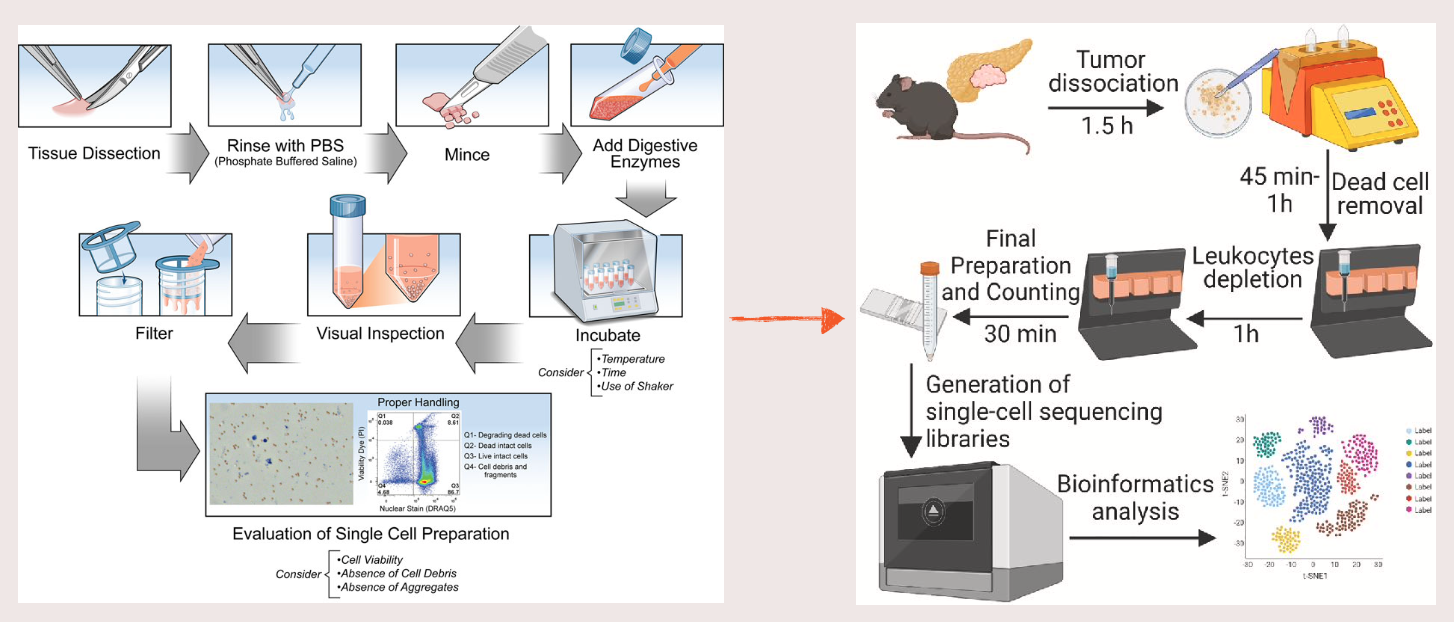
\includegraphics[width=0.5\textwidth]{images/Screenshot_1.png}
\caption{STAR Protocols 2, 100989, December 17, 2021}
\end{figure}

\hypertarget{single-cell-sorting}{%
\subsection{Single cell sorting}\label{single-cell-sorting}}

While working with rare cells or genetically modified cells, it is
required to apply \textbf{FACS} (Fluorescent Activated Cell Sorting),
where cells are fluorescently labelled and driven by pressure in a tube
where laser excites cells and a detector reads chemical properties.
Finally, cells are sorted through deflector plates, included in a
droplet and inserted in collection tubes. The overall procedure is long
and stress-inducing, hence cells could have changes in gene expression
profile (possible solution: freeze a part of the samples for final
comparison).

\begin{figure}
\centering
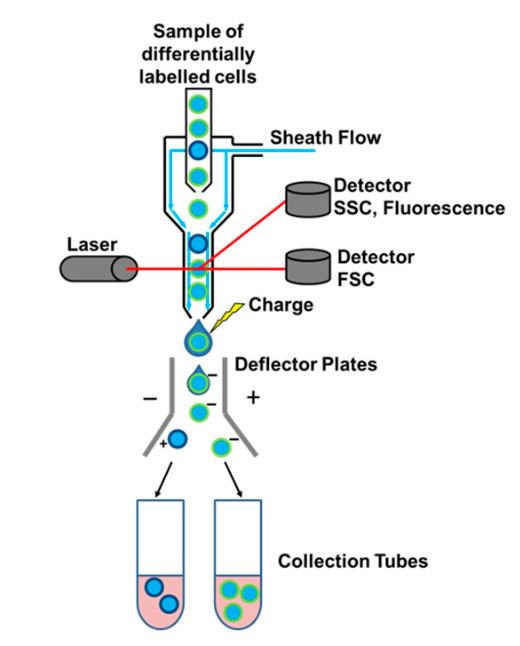
\includegraphics[width=0.3\textwidth]{images/Screenshot_2.png}
\caption{G Pfister et al., J Immunol Meth 487 (2020) 112902 }
\end{figure}


\textbf{Microfluidic sorters} provide a commercial solution to the
issue. They work in a sterile environment, are based on disposables,
avoid cross contaminations and apply a gentle analysis. Through the
\emph{actuator,} cells are mechanically accompanied to the right channel
without stress induction. Examples:

\begin{itemize}
\tightlist
\item
  LeviCell, LevitasBio: label free system exploiting the magnetic
  properties of nanoparticles in cells for sorting. Drawback: small
  input channels, only a small number of cells is allowed.
\end{itemize}

\hypertarget{sample-collection-and-preservation}{%
\subsection{Sample collection and
preservation}\label{sample-collection-and-preservation}}

With the advent of molecular pathology, hospitals started to collect
fresh and frozen tissue in addition to FFPE-preserved tissue
traditionally used in immunohistochemistry. From these sample, it is
possible to isolate both nuclei and cells according to the techniques.
In order to maintain samples in time, freezing is a feasible solution,
as cells can be cultured again after many years.

\begin{figure}
\centering
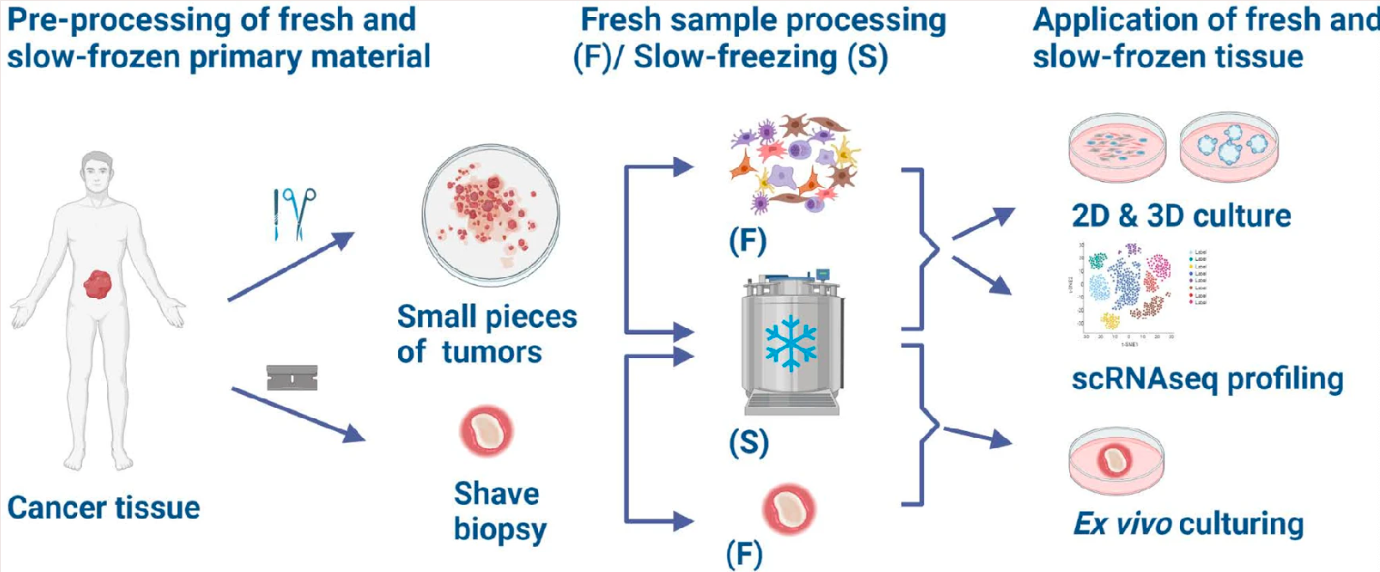
\includegraphics[width=0.5\textwidth]{images/Screenshot_3.png}
\caption{G. Restivo et al. Commun Biol 5, 1144 (2022)}
\end{figure}

Keep in mind that different assays require different input materials:

\begin{itemize}
\tightlist
\item
  protein expression: whole cells
\item
  gene expression: whole cell nuclei
\item
  chromatin accessibility: nuclei
\end{itemize}

Determining your required input can help you determine what collection
and preservation method is most suitable for your sample type.

\hypertarget{xgenomics}{%
\section{10xGenomics}\label{xgenomics}}

Three main pillar technologies:

\begin{enumerate}
\def\labelenumi{\arabic{enumi}.}
\tightlist
\item
  Chromium Single Cell: NGS readout
\item
  Visium Spatial: NGS readout
\item
  Xenium In Situ: microscopy-based readout
\end{enumerate}

In \textbf{feature barcode technology} we aim at combining different
cells in the same sequencing run through cell multiplexing, cell surface
protein or CRISPR screening. Older machines run in manual mode, while
the more recent Chromium Connect is automated and able to perform gene
expression immune profiling.

\hypertarget{feature-barcode-technology}{%
\subsection{Feature barcode
technology}\label{feature-barcode-technology}}

In the standard approach, we find 3.6M barcodes, while in low throughput
(a bit cheaper) 9.2K barcodes. The capture sequence is directed to
antibody or guide RNA for gene activity disruption.

\begin{figure}
\centering
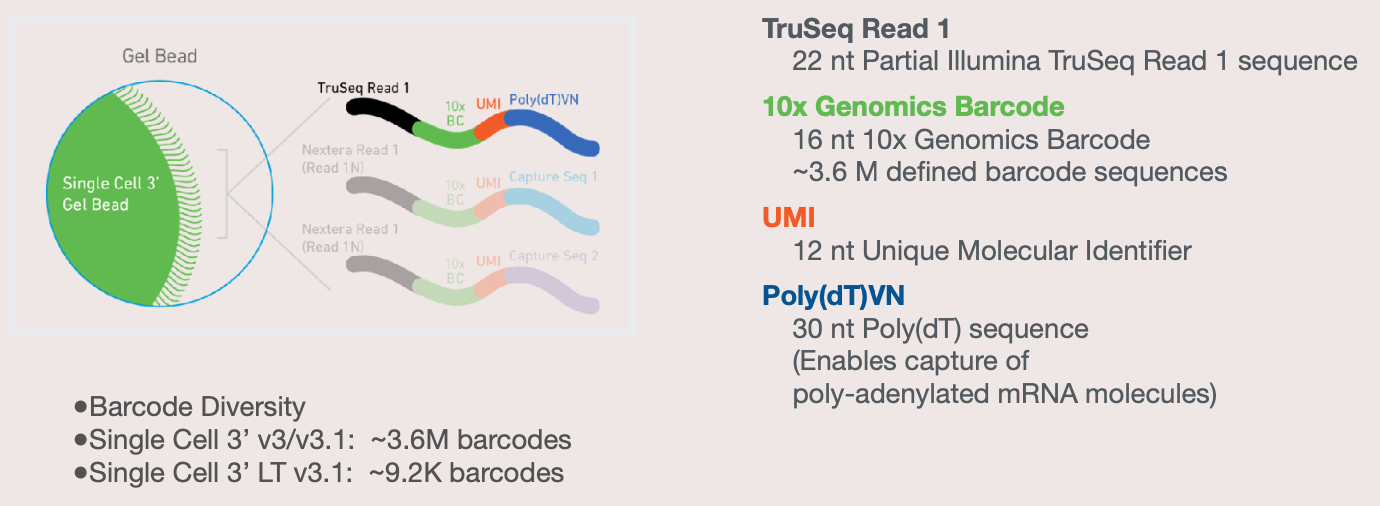
\includegraphics[width=0.5\textwidth]{images/Screenshot_4.png}
\caption{10x Genomics}
\end{figure}

Samples are inserted in a chip with wells.

\begin{figure}
\centering
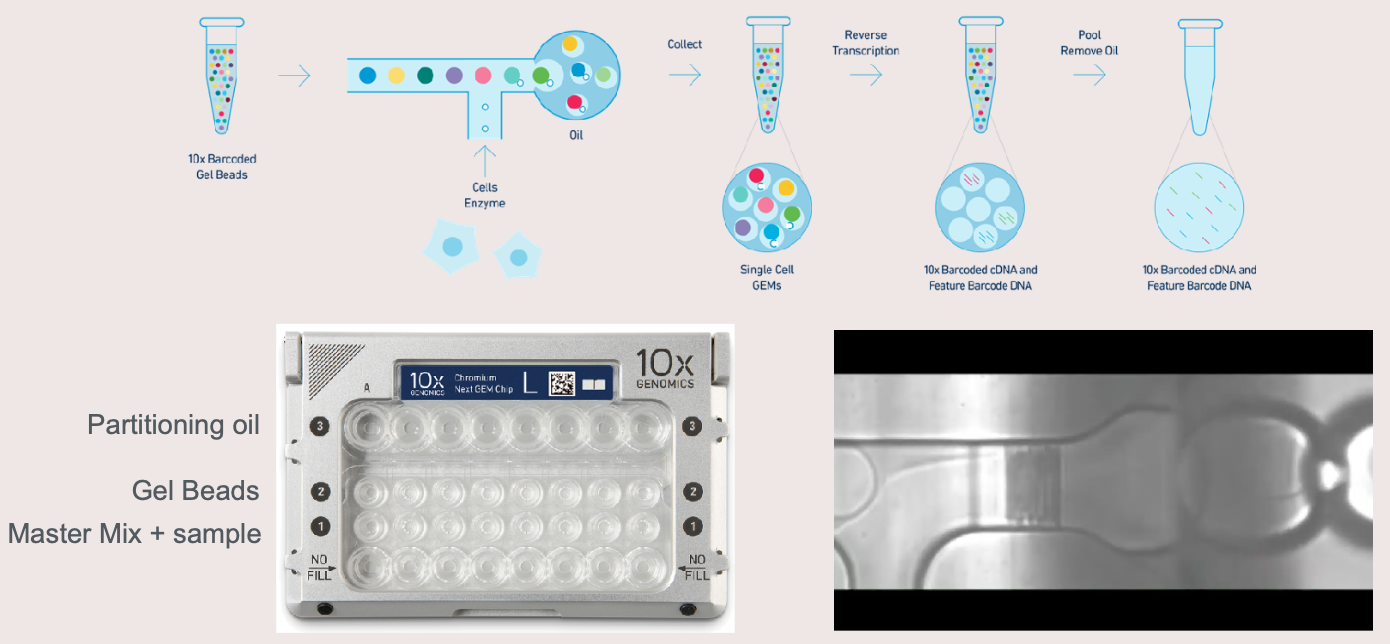
\includegraphics[width=0.5\textwidth]{images/Screenshot_5.png}
\caption{10x Genomics}
\end{figure}

\textbf{Bio-Rad vs 10x Genomics patent war:} develoment of digital PCR
by Quantalife, bought by Bio-Rad.

\hypertarget{single-cell-gene-expression-workflow}{%
\subsection{Single cell gene expression
workflow}\label{single-cell-gene-expression-workflow}}

\begin{enumerate}
\def\labelenumi{\arabic{enumi}.}
\item
  GEM

  \begin{figure}
  \centering
  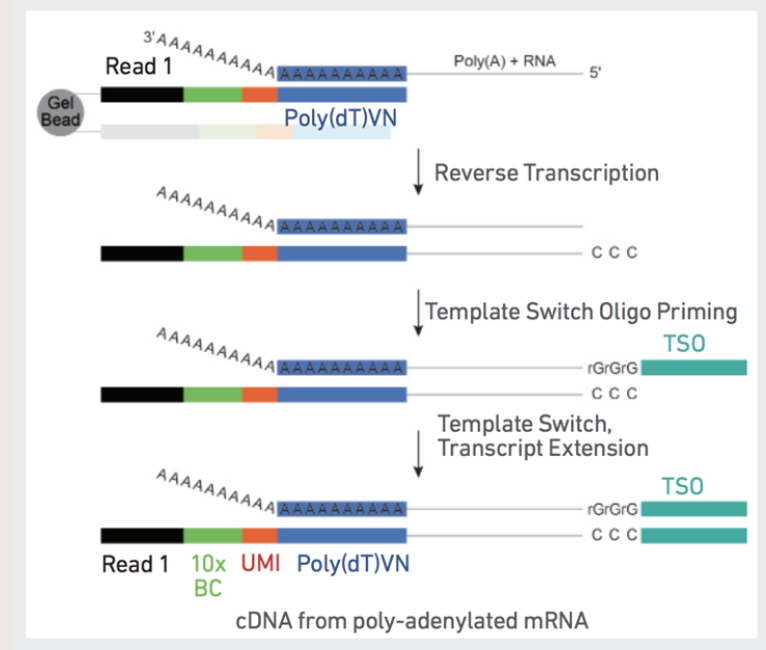
\includegraphics[width=0.5\textwidth]{images/Screenshot_6.png}
  \caption{10x Genomics}
  \end{figure}
\item
  GEM breakage

  \begin{figure}
  \centering
  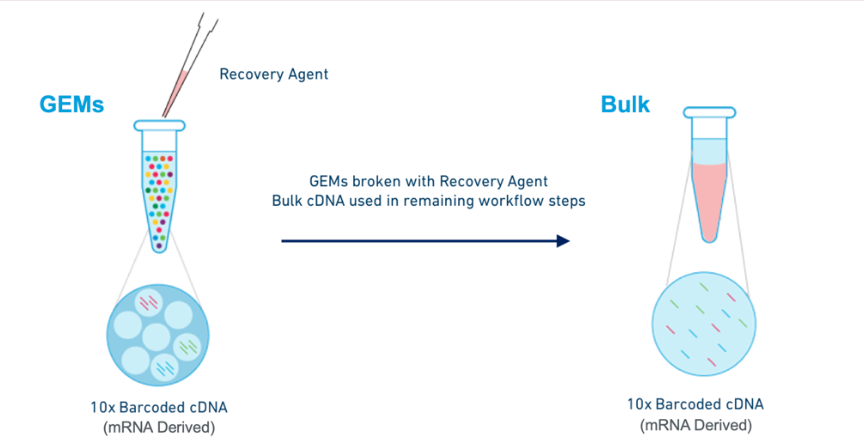
\includegraphics[width=0.5\textwidth]{images/Screenshot_7.png}
  \caption{10x Genomics}
  \end{figure}
\item
  cDNA amplification and library construction

  \begin{figure}
  \centering
  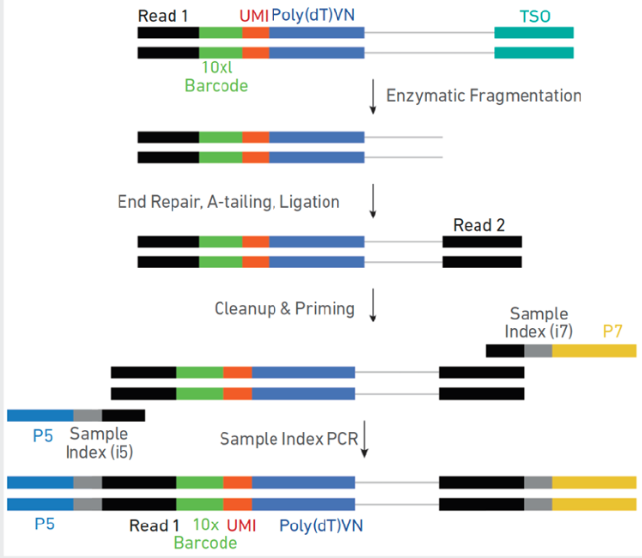
\includegraphics[width=0.5\textwidth]{images/Screenshot_8.png}
  \caption{10x Genomics}
  \end{figure}
\end{enumerate}

\hypertarget{chip-based-single-cell-separator}{%
\subsection{Chip-based single cell
separator}\label{chip-based-single-cell-separator}}

Chip-based single cell separator → iCELL8 cv (TAKARA) 72x72 wells, check
the quality by inspection through a microscope. Very low volumes, we
should have no air in the solution. Upper limit for nozzle is higher
than 10x, so it is possible to analyze bigger cells e.g.~Schwann cells
or cardiomyocytes. With this technique, reagents are only dispensed in
selected wells.

\begin{figure}
\centering
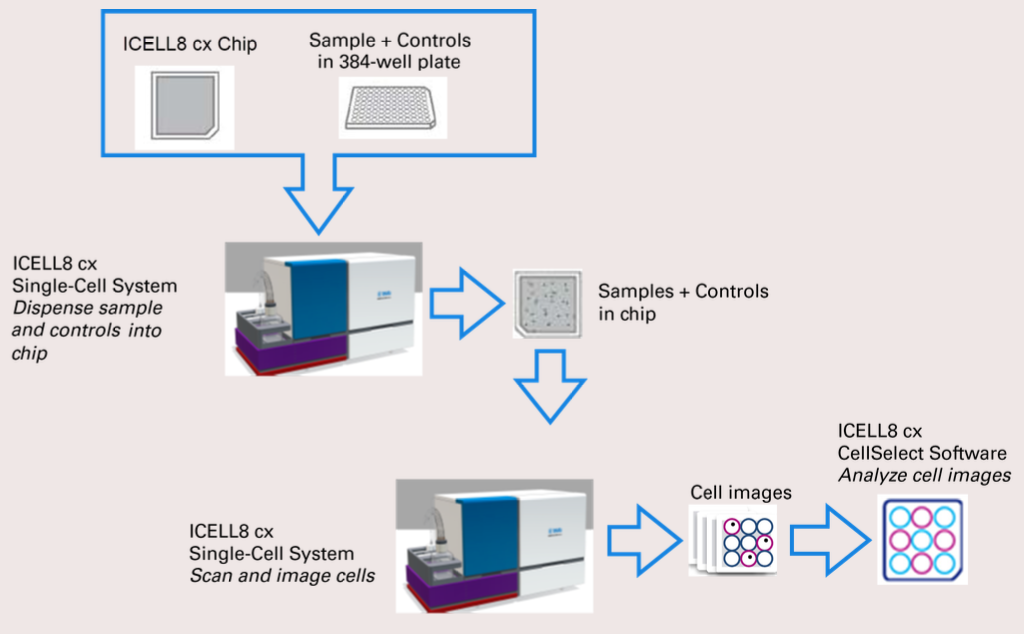
\includegraphics[width=0.5\textwidth]{images/Screenshot_9.png}
\caption{iCELL8cx cell scan workflow}
\end{figure}

\hypertarget{hive-scrnaseq-solution}{%
\subsection{HIVE scRNAseq
Solution}\label{hive-scrnaseq-solution}}

The HIVE collector is composed of a membrane with wells. The technology
is based on pore properties and gravity sorting (more gentle approach)
by the usage of vortex. It is possible to integrate sample storage in
the workflow with freezing. The main advantage is the lack of
specialized instrumentation, but we have a huge limit on the number of
analyzable cells.
